\documentclass[preprint,11pt,authoryear]{elsarticle}
\pdfoutput=1
\pdfminorversion=4 %had problems submitting a v1.5 pdf file with J Neurosci Methods
\usepackage{graphicx}
\usepackage{amsmath}
\usepackage{esint}
\usepackage{amssymb}
\usepackage{lineno}
\usepackage[T1]{fontenc}
\usepackage[utf8]{inputenc}
\usepackage[english]{babel}
\usepackage[]{algorithm}
\usepackage[noend]{algpseudocode}
%% natbib.sty is loaded by default. However, natbib options can be
%% provided with \biboptions{...} command. Following options are
%% valid:

%%   round  -  round parentheses are used (default)
%%   square -  square brackets are used   [option]
%%   curly  -  curly braces are used      {option}
%%   angle  -  angle brackets are used    <option>
%%   semicolon  -  multiple citations separated by semi-colon
%%   colon  - same as semicolon, an earlier confusion
%%   comma  -  separated by comma
%%   numbers-  selects numerical citations
%%   super  -  numerical citations as superscripts
%%   sort   -  sorts multiple citations according to order in ref. list
%%   sort&compress   -  like sort, but also compresses numerical citations
%%   compress - compresses without sorting
%%
%% \biboptions{comma,round}

% \biboptions{}

\bibliographystyle{elsarticle-harv}
\biboptions{square}

\renewcommand\familydefault{\sfdefault}
\usepackage[scaled]{helvet}

\usepackage{units}
\usepackage[usenames, dvipsnames]{xcolor}

\usepackage{soul}
\usepackage{placeins}

\usepackage{nameref}
\usepackage[pdftex,breaklinks=true,colorlinks=true,linkcolor=blue,citecolor=blue,urlcolor=blue,filecolor=blue,pdffitwindow,backref=true,pagebackref=false,bookmarks=true,bookmarksopen=true,bookmarksnumbered=true]{hyperref}
\usepackage[plain]{fancyref}
\usepackage{array}
\usepackage{multirow}

% Text layout
%\hoffset 2 cm
\topmargin 0.0cm
\oddsidemargin 0.5cm
\evensidemargin 0.5cm
\textwidth 16cm 
\textheight 21cm

%custom color for \hlc
\newcommand{\hlc}[2][yellow]{ {\sethlcolor{#1} \hl{#2}} }
\newcommand{\hlb}[2][blue]{ {\sethlcolor{#1} \hl{#2}} }
\newcommand{\hlr}[2][Maroon]{ {\sethlcolor{#1} \hl{#2}} }
\newcommand{\hlj}[2][OliveGreen]{ {\sethlcolor{#1} \hl{#2}} }
\newcommand{\hlR}[2][red]{ {\sethlcolor{#1} \hl{#2}} }
\newcommand{\hlp}[2][Purple]{ {\sethlcolor{#1} \hl{#2}} }
\newcommand{\hlt}[2][Tealblue]{ {\sethlcolor{#1} \hl{#2}} }

%boxes and highlight color for text updates, personified!
\newcommand{\ghnote}[1]{\color{white}{\hlb{GH: #1 }}\color{black}}
\newcommand{\ghtxt}[1]{{\color{blue}#1}}
\newcommand{\gtenote}[1]{\color{white}{\hlR{GTE: #1 }}\color{black}}
\newcommand{\gen}[1]{\color{white}{\hlR{GTE: #1 }}\color{black}}
\newcommand{\gtetxt}[1]{{\color{red}#1}}
\newcommand{\gex}[1]{{\color{red}#1}}
\newcommand{\genn}[1]{{\color{orange}#1}}

\newcommand{\tvnnote}[1]{\color{white}{\hlj{TVN: #1 }}\color{black}}
\newcommand{\tvntxt}[1]{{\color{OliveGreen}#1}}

\newcommand{\snnote}[1]{\color{white}{\hlp{SN: #1 }}\color{black}}
\newcommand{\sntxt}[1]{{\color{Purple}#1}}
\newcommand{\slntxt}[1]{{\color{RoyalPurple}#1}}


%fancy ref formatting
\Frefformat{plain}{\fancyreffiglabelprefix}{Fig~#1}
\newcommand*{\Frefsecshortname}{Section}%
\Frefformat{plain}{\fancyrefseclabelprefix}{\Frefsecshortname~#1}
\Frefformat{plain}{\fancyrefeqlabelprefix}{Eq~(#1)}

%tables as in Nordlie et al. (2009)
\usepackage{tabularx}
\usepackage{colortbl}
\usepackage{morefloats}

%table formatting
\newcommand{\modelhdr}[3]{%
   \multicolumn{#1}{|l|}{%
     \color{white}\cellcolor[gray]{0.0}%
     \textbf{\makebox[0pt]{#2}\hspace{0.5\linewidth}\makebox[0pt][c]{#3}}%
   }%
}
\newcommand{\parameterhdr}[3]{%
   \multicolumn{#1}{|l|}{%
     \color{black}\cellcolor[gray]{0.8}%
     \textbf{\makebox[0pt]{#2}\hspace{0.5\linewidth}\makebox[0pt][c]{#3}}%
   }%
}
\def\tabspace{0.5ex}

\usepackage{float}
\floatstyle{plaintop}
\restylefloat{table}

\journal{nobody}


% redefinition of \author{•} because of bug (reset of \@corref missing), taken from:
% http://tex.stackexchange.com/questions/116515/elsarticle-frontmatter-corresponding-author
%
\makeatletter
\def\@author#1{\g@addto@macro\elsauthors{\normalsize%
    \def\baselinestretch{1}%
    \upshape\authorsep#1\unskip\textsuperscript{%
      \ifx\@fnmark\@empty\else\unskip\sep\@fnmark\let\sep=,\fi
      \ifx\@corref\@empty\else\unskip\sep\@corref\let\sep=,\fi
      }%
    \def\authorsep{\unskip,\space}%
    \global\let\@fnmark\@empty
    \global\let\@corref\@empty  %% Added
    \global\let\sep\@empty}%
    \@eadauthor={#1}
}
\makeatother

% - mine pakker -
\usepackage[exponent-product = \cdot]{siunitx}
\usepackage[colorinlistoftodos]{todonotes}
\usepackage[normalem]{ulem} % strikethroughs \sout{Hello World}
\usepackage{caption}
\usepackage{booktabs} % to make nice tables
\graphicspath{{Figures/}} %Setting the graphicspath
\usepackage{caption}
\usepackage{subcaption}

% - mine kommandoer - 


\begin{document}

\begin{frontmatter}

%% Title, authors and addresses

\title{Computing extracellular electrical potentials from neuronal simulations} 

%% use the tnoteref command within \title for footnotes;
%% use the tnotetext command for the associated footnote;
%% use the fnref command within \author or \address for footnotes;
%% use the fntext command for the associated footnote;
%% use the corref command within \author for corresponding author footnotes;
%% use the cortext command for the associated footnote;
%% use the ead command for the email address,
%% and the form \ead[url] for the home page:
%%
%% \title{Title\tnoteref{label1}}
%% \tnotetext[label1]{}
%% \author{Name\corref{cor1}\fnref{label2}}
%% \ead{email address}
%% \ead[url]{home page}
%% \fntext[label2]{}
%% \cortext[cor1]{}
%% \address{Address\fnref{label3}}
%% \fntext[label3]{}

%% use optional labels to link authors explicitly to addresses:
%% \author[label1,label2]{<author name>}
%% \address[label1]{<address>}
%% \address[label2]{<address>}

\author{Geir Halnes\fnref{label1,label2}}
\author{Torbj\o{}rn V. Ness \fnref{label1}}
\author{Solveig N\ae{}ss\fnref{label2}}
\author{Klas Pettersen \fnref{label3}}
\author{Gaute T. Einevoll\corref{cor1}\fnref{label1,label2,label4}}

\address[label1]{Faculty of Science and Technology, Norwegian University of Life Sciences, {{\AA}}s, Norway}
\address[label2]{Center for Integrative Neuroplasticity, University of Oslo, Oslo, Norway}
\address[label3]{Norwegian Artificial Intelligence Research Consortium, Oslo, Norway}
\address[label4]{Department of Physics, University of Oslo, Oslo, Norway}

\cortext[cor1]{correspondence: \href{geir.halnes@nmbu.no}{gaute.einevoll@nmbu.no}}

%%%%%%%%%%%%%%%%%%%%%%%%%%%%%%%%%%%%%%%%%%%%%%%%%%
%%%%%%%%%%%%%%%%%%%%%%%%%%%%%%%%%%%%%%%%%%%%%%%%%%


\begin{abstract}
%% Text of abstract
\ghnote{Vet ikke hva forfatterordningen skal vaere, men vi faar se det an etter hvert, og bestemme utifra hvem som har jobbet mest med manus. For oeyeblikket leder jeg, men jeg tror jeg satser paa at kanskje Torbjoern fosser forbi etter hvert.}
\tvnnote{Just to be sure: If we make figures for this chapter, we have the right to re-use those wherever we like?}
\tvnnote{Giugliano: max 15-20 pages, by February 2020 }
\end{abstract}

\begin{keyword}
extracellular potentials \sep LFP \sep EEG \sep ECoG \sep electrodiffusion
%% keywords here, in the form: keyword \sep keyword

%% MSC codes here, in the form: \MSC code \sep code
%% or \MSC[2008] code \sep code (2000 is the default)
\end{keyword}

\end{frontmatter}

\tableofcontents

%%%%%%%%%%%%%%%%%%%%%%%%%%%%%%%%%%%%%%%%%%%%%%%%%%
%%%%%%%%%%%%%%%%%%%%%%%%%%%%%%%%%%%%%%%%%%%%%%%%%%
%% Start line numbering here if you want
\linenumbers

\section{Introduction}
\tvnnote{Gaute skriver dette}
\label{sec:introduction}

\ghnote{First something about why we are interested in electrical fields and some historical perspectives. Perhaps Gaute should write this.}

\ghnote{End intro with bridge to theory-section. Probably we should add some older references to VC-theory?}


Very important to model what you measure, and measure what you model \citep{Einevoll2019, Maki-marttunen2019}


Within the field of computational neuroscience, there has been a strong focus on modelling the membrane potential dynamics of morphologically complex neurons. Such simulations involve computing the transmembrane currents in all neuronal segments. This book chapter explains how one, based on knowing the transmembrane currents, can compute the electrical potential in the extracellular space surrounding the active neurons. 

The link between membrane currents and the extracellular potential is of course mediated by electrical currents. Electrical currents in the brain are mediated by the movement of ions, and it is these currents that a recording electrode pick up.  A net electrical current through the extracellular space of the brain could in principle include several components, such as (1) a drift component (ions migrate in electrical fields), (2) a diffusion component (ions diffuse), (3) an advective component (extracellular fluid flow drags ions along), and (4) a displacement component (ions pile up and changes the local charge density). Since the extracellular bulk fluid has very fast relaxation times and is very close to electroneutral, the latter two current components (3-4) are extremely small and are typically neglected \citep{Grodzinsky2011, Gratiy2017}. The diffusive component (3) is acknowledged to play an important role for voltage dynamics on a tiny spatial scale, such as in synaptic clefts or in the close vicinity of neuronal membrane, where ion concentrations can change dramatically within very short time \citep{Savtchenko2017, Pods2017}. At the level of tissue, it is commonly believed that the diffusive current is much smaller than the drift current, so that even diffusive currents are typically neglected \citep{Holt1999, Pettersen2008a}. This is often a useful approximation, since modeling of electrodiffusive processes is computationally expensive and may not be feasible for large and complex systems. However, if concentration gradients are present, diffusive currents could in principle affect measurable extracellular potentials \citep{Halnes2016, Halnes2017, Solbra2018}, and in scenarios involving dramatic shifts in extracellular concentrations, such as spreading depression and related pathologies, diffusive effects are likely to be of key importance for shaping the extracellular potential \citep{Almeida2004, OConnell2016}.

We start this book chapter by giving an overview of the theory used for forward modellng of extracellular potentials, and introduce the mathematical frameworks and software tools that can be used for such modelling. We start the theory-part at the rather fundamental level of electrodiffusive ion concentration dynamics, and derive an electrodiffusive framework for predicting the dynamics of the extracellular ion concentrations and potential. We next show how this theory can be reduced to the simpler, and more common VC-theory if we assume that the diffusive component is negligible. 

\begin{figure}[!ht]
\begin{center}
\includegraphics[width=0.8\textwidth]{cortex_multipop_arial_font}
\end{center}
\caption{\textbf{LFP, ECoG, EEG and MEG.} The same basic building blocks, that is, currents caused by large numbers of synaptic input are contributing to several different measurable signals.}
\label{fig:multimodal}
\end{figure}

Motivation: Simulated test-data for benchmarking
Spike-sorting: \cite{Hagen2016, Buccino2019}, CSD: \cite{Pettersen2006, Potworowski2012, Ness2015}, 
Location and Cell type: \citep{DelgadoRuz2014, Buccino2018}, 
LPA

\section{%Theory: 
From electrodiffusion to volume conductor theory}
\label{sec:theory}
We start at the very smallest of scales considered in neuroscience, by describing the fundamentals of how ions are moving through the brain under the influence of electric fields and concentration gradients. Building on this, we describe how ionic currents affect the electric extracellular potentials inside neural tissue, like the local field potential (LFP), and furthermore, how they cause electric potentials and magnetic fields that are measurable even outside of the head.

\subsection{Ion concentration dynamics}
\label{sec:eldiff}
In electrodiffusive processes, the flux density of an ion species $k$ is given by \cite{Koch1999}:
\begin{equation}
{\bf J_k} = - D_{k} {\bf \nabla} c_{k} - \frac{D_k z_k c_k}{\psi} {\bf \nabla} \phi,
\label{eq:JNP}
\end{equation}
where the first term on the right is Fick's law for the diffusive flux density $J_{k}^\text{diff}$, and the second term is the drift flux density $J_{k}^\text{drift}$, which expands Fick's law in the case where the diffusing particles also move due to electrostatic forces with a mobility $D_k/\psi$ (cf. the Einstein-relation \cite{Mori2008}). Here $D_{k}$ is the diffusion coefficient of ion species $k$, $\phi$ is the electric potential, $z_{k}$ is the valency of ion species $k$, and $\psi=RT/F$ is defined by the gas constant ($R$), Faraday's constant ($F$)  and the temperature ($T$). The ion concentration dynamics of a given species is then given by the Nernst-Planck continuity equation:

\begin{equation}
\frac{\partial c_k}{\partial t} = - {\bf \nabla} \cdot {\bf J_k} + f_k = {\bf \nabla} \cdot \left[ D_k {\bf \nabla} c_k + \frac{D_k z_k c_k}{\psi} {\bf \nabla} \phi \right] + f_k
\label{eq:NP}
\end{equation}
where $f_k$ represents any source term in the system, such as e.g., an ionic transmembrane current source   \cite{Solbra2018}. 

In order the solve a set (i.e., one for each ion species present) of equations like (\ref{eq:NP}), one needs an expression for the electrical potential $\phi$. There are two main approaches to this. The physically most detailed approach is to use the Poisson-Nernst-Planck (PNP) formalism \citep{Leonetti1998, Leonetti2004, Lu2007, Lopreore2008, Nanninga2008, Pods2013, Gardner2015}. Then $\phi$ is determined from Poisson's equation from electrostatics, 
\begin{equation}
\nabla^2 \phi = -\rho/\epsilon, 
\label{eq:poisson}
\end{equation}
where $\epsilon$ is the permittivity of the system, and $\rho$ is the charge density associated with the ionic concentrations, as given by:
\begin{equation}
\rho = F \sum_k z_k c_k.
\label{eq:F}
\end{equation}
An alternative, more computationally efficient approach is to replace the Poisson equation with the simplifying approximation that the bulk solution is electroneutral \citep{Mori2008, Mori2009, Mori2009a, Mori2011, Halnes2015, Halnes2013, Pods2017, Niederer2013, OConnell2016, Solbra2018}, which is a good approximation on spatiotemporal scales larger than micrometers and microseconds \citep{Grodzinsky2011, Pods2017, Solbra2018}. 

Both the PNP formalism and the electroneutral formalism allow us to compute the dynamics of ion concentrations and the electrical potential in the extracellular space of neural tissue containing an arbitrary set of neuronal and glial current sources. For example, in recent work, a version of the electroneutral formalism was developed into a framework for computing the extracellular dynamics (of $c_k$ and $\phi$) in a 3D space surrounding morphologically complex neurons simulated with the NEURON simulation tool \citep{Solbra2018}. However, both the PNP and electroneutral formalisms keep track of the spatial distribution of ion concentrations, and as such they require a suitable meshing of the 3D space, and numerical solutions based on finite difference- or finite element methods. In both cases, simulations can become very heavy, and for systems at a tissue level, the computational demand may become incommensurable. For that reason, there is much to gain from deriving simpler frameworks where effects of ion concentration dynamics are neglected, since, for many scenarios, this may be a good approximation. Below, we will derive these simpler frameworks using the Nernst-Planck fluxes (eq. \ref{eq:JNP}) as a starting point, as this approach will make the involved approximations transparent.

\subsection{Electrodynamics}
If we multiply eq. \ref{eq:JNP} by $F\cdot z_k$ and take the sum over all ion species, we get an expression for the net electrical current density due to all particle fluxes:

\begin{equation}
{\bf I} = - \sum_k{F z_k D_{k}{\bf \nabla} c_{k}} - \sigma {\bf \nabla}{\phi}
\label{eq:INP}
\end{equation}
where the first term is the diffusive current density $I^\text{diff}$ and the second term is the drift current density$I^\text{drift}$. We have here identified the conductivity $\sigma$ of the medium as \citep{Koch1999}:
\begin{equation}
\sigma = F\sum_{k} \frac{\tilde{D}_{k} z_{k}^2}{\psi}c_{k}.
\label{eq:sigma}
\end{equation}
Current conservation in the extracellular space implies that:
\begin{equation}
{\bf \nabla} \cdot {\bf I} = - \sum_k{F z_k D_{k}\nabla^2 c_{k}} - {\bf \nabla} \cdot (\sigma {\bf \nabla} \phi) = - CSD,
\label{eq:CSD}
\end{equation}
where $CSD$ denotes the current source density, reflecting e.g., local neuronal or glial transmembrane currents. We note that this is essentially equivalent to eq. \ref{eq:NP} at the level of single ion species, with the exception eq. \ref{eq:NP} contained a term $\partial c_k/ \partial t$ for accumulation of ion species $k$, while eq. \ref{eq:CSD} does \emph{not} contain a corresponding term ($\partial \rho/ \partial t$) for charge accumulation. Hence, in eq. (\ref{eq:CSD}) it is implicitly assumed that the extracellular bulk solution is electroneutral \citep{Solbra2018}. We note that in general, the $CSD$ term includes both ionic transmembrane currents and transmembrane capacitive currents, and that the latter means that the local charge accumulation building up the transmembrane potential still occurs in the membrane Debye-layer.

Note that if we assume all concentrations to be constant in space, the diffusive term vanishes, and eq. (\ref{eq:CSD}) reduces to:
\begin{equation}
{\bf \nabla} \cdot (\sigma {\bf \nabla} \phi) = - CSD,
\label{eq:CSDstandard}
\end{equation}
This the standard expression used in current source density (CSD) theory \citep{Mitzdorf1985, Nicholson1975, Pettersen2006}, where spatially distributed recordings of $\phi$ are used to make theoretical predictions of underlying current sources. When using Eq. \ref{eq:CSDstandard}, it is implicitly assumed that the Laplacian of $\phi$ exclusively reflects transmembrane current sources, and that it is not contributed to by diffusive processes. 

As eq. (\ref{eq:CSD}) indicates, also diffusive processes can in principle contribute to the Laplacian of $\phi$, and if present, they could give rise to a non-zero Laplacian of $\phi$ even in the absence of neuronal sources ($CSD = 0$). Previous computational \sntxt{studies} have predicted that effects of diffusion on extracellular potentials are not necessarily small, but tend to be very slow, meaning that they will only affect the very low-frequency components of $\phi$ \citep{Halnes2016, Halnes2017}. This is due to the diffusive current being a direct function of ion concentrations $c_k$, which on a large spatial scale typically vary on a much slower time scale (seconds-minutes) than the fluctuations in $\phi$ that we commonly are interested in (milliseconds-seconds). Furthermore, electrodes used to record $\phi$ typically have a lower cutoff frequency of 0.1-1Hz \citep{Einevoll2013}, which means that most of the tentative diffusive contribution will be filtered out from experimental recordings. It may therefore be a good approximation to neglect the diffusive term, except in the case of pathologically dramatic concentration variations. For the rest of this chapter, we shall do so, and assume that electrodynamics in neural tissue can be determined by eq.~(\ref{eq:CSDstandard}).

\subsection{Volume conductor theory}
\label{sec:VC_theory}
In simulations of morphologically complex neurons, we typically compute a set of transmembrane current sources for each neuronal segment \citep{Koch1999}. Commonly, one assumes that the extracellular potential does not effect \snnote{affect?} the neurons (i.e., no ephaptic coupling), since extracellular potentials are typically much smaller than the membrane potential of $\sim$-70~mV. 
By assuming that the tissue medium is a volume conductor \citep{Holt1999, Linden2014}, one can then use the standard CSD-equation (eq. \ref{eq:CSDstandard}) to perform a forward modeling of the extracellular potential at each point in space surrounding the neuron(s). 

If we consider the simplest possible case of a single point current source $I_1$ in ${\bf r}=0$ in an isotropic medium, the current density $I = -\sigma \nabla \phi$ through a spherical shell with area $4\pi r^2$ must equal $I_1/4\pi r^2$. 
\snnote{It would be nice with a clearer distinction between current and current density.. What about using uppercase I for current and lowercase i for current density?}
Due to the spherical symmetry of the problem, $\nabla \phi = d\phi/dr$, and integration with respect to $r$ gives us:

\begin{equation}
\phi = \frac{I_1}{4\pi \sigma r},
\label{eq:pointsource}
\end{equation}
where $r$ is the distance from the source. If we have several point-current sources, $I_{1}, I_2, I_3, ... $ in locations ${\bf r_1}, {\bf r_2}, {\bf r_3} ... $), their contributions add up due to the linearity assumption, and the potential in a point ${\bf r}$ is given by:

\begin{equation}
\phi({\bf r}) = \frac{I_1}{4\pi  \sigma {\bf |r-r_1|}} + \frac{I_2}{4\pi  \sigma {\bf |r-r_2|} } + \frac{I_3}{4\pi  \sigma {\bf |r-r_3|} } + ... = \sum_k \frac{I_k}{4\pi  \sigma {\bf |r-r_k|} }.
\label{eq:VCtheory}
\end{equation}

Eq.~\ref{eq:VCtheory} is often referred to as the point-source approximation \citep{Holt1999, Pettersen2008a}, since the membrane current from a neuronal segment is assumed to enter the extracellular medium in a single point. An often used further development is obtained by integrating eq.~\ref{eq:VCtheory} along the segment axis, corresponding to the transmembrane current being evenly distributed along the segment axis, giving the line-source approximation \citep{Holt1999, Linden2014}.

\snnote{multipole expansion and current dipole approximation}


%\slntxt{
%Imagine that we want to compute the electric potential from a volume of current sinks and sources. The obvious choice would be to apply the point-source approximation, eq.~\eqref{eq:VCtheory}.
%	
%The point-source approximation can also be reformulated into an infinite series called the multipole expansion for current sources:
%
%\begin{equation}
%\Phi(R) = \frac{C_{monopole}}{R} + \frac{C_{dipole}}{R^2} + \frac{C_{quadrupole}}{R^3} + \frac{C_{octupole}}{R^4} + ... .
%\end{equation}
%The multipole expansion will precisely give us the electric potential at a distance $R$ away from the volume, when $R$ is larger than the maximal radius of the volume: $R > |r_{vol}|_{max}$.
%
%The multipole expansion is apparently not so useful in it's original form, but let us:
%}

\sntxt{
By reformulating Eq.~\eqref{eq:VCtheory}, we find that the electric potential from a volume containing a combination of current sinks and sources, can be precisely described by the multipole expansion \citep{Nunez2006}:

\begin{equation}\label{eq:multipole}
\Phi(R) = \frac{C_{monopole}}{R} + \frac{C_{dipole}}{R^2} + \frac{C_{quadrupole}}{R^3} + \frac{C_{octupole}}{R^4} + ...
\end{equation}
when the distance from the center of the volume to the measurement point is larger than the maximal distance from volume center to source [cite - find Jackson!].

In neural tissue, current monopoles are unphysical due to current conservation and the quadrupole, octopole and higher-order contributions decay rapidly with distance $R$. Consequently, the multipole expansion can be approximated by the dipole contribution for large distances, a simplification known as the current dipole approximation \citep{Nunez2006}:
\begin{equation}\label{eq:CDA}
\Phi(\mathbf{R}) \approx \frac{1}{4 \pi \sigma} \frac{|\mathbf{p}| \cos \theta}{R^2}.
\end{equation}
Here, $\mathbf{p}$ is the current dipole moment and $\theta$ is the angle between the current dipole moment and the distance vector $\mathbf{R}$. The current dipole moment can be found by summing up all the transmembrane currents from a neuron \citep{Pettersen2008, Pettersen2014, Nunez2006}: 
\begin{equation}\label{eq:dipole}
\mathbf{p} = \sum_{k=1}^N I_k \mathbf{r}_k.
\end{equation}
For a current sink $-I$ at location $\mathbf{r}_1$ and a current source $I$ at location $\mathbf{r}_2$, the current dipole moment can be formulated as $\mathbf{p} = -I\mathbf{r}_1 + I\mathbf{r}_2 = I(\mathbf{r}_2 - \mathbf{r}_1) = I\mathbf{d}$, where $\mathbf{d}$ is the distance vector between the current sink and the current source, giving the length $d$ and direction of the current dipole. As mentioned above, the current dipole approximation is applicable when we are in the far-field limit, that is when $R$ is much larger than the dipole length: $R > 3d$ or $R > 4d$ \citep{Nunez2006}.

The point-source approximation, Eq. \ref{eq:VCtheory} (or the line-source version of it), and the current dipole approximation, Eq.~\eqref{eq:CDA} represent} volume conductor theory in its simplest form, and \sntxt{are} based on a set of assumptions, some of which may be relaxed for problems where it is relevant: 

\begin{enumerate}

\item {\bf Quasi-static approximation of Maxwell's equations:} Terms with time derivative of the electrical and magnetic fields are neglected. This approximation appears to be well-justified for the relatively low frequencies relevant for brain signals, below about 10 kHz \citep{Nunez2006}.

\item {\bf Linear extracellular medium:} Linear relationship ($\bf{I} = -\sigma {\nabla \phi}$) between the current density ${\bf I}$\tvnnote{I would have preferred J to mean current density and I total currents. Will this make things messy other places?} \ghnote{Maybe it messes things up, since I used $J_k$ for fluxes earlier.} and the electrical field, $\nabla \phi$. This is essentially Ohm's law for volume conductors, and the relation is constitutive, meaning that it is observed in nature rather than derived from any physical principle \citep{Nunez2006, Pettersen2012}.

\item {\bf Frequency independent conductivity:} Capacitive effects in neural tissue are assumed to be negligible compared to resistive effects in volume conduction. This approximation seems to be justified for the relevant frequencies in extracellular recordings \citep{Logothetis2007, Miceli2017, Ranta2017}, see Fig.~\ref{fig:freq_dep}. Note that it is possible to expand the formalism to include a frequency dependent conductivity \citep{Tracey2011, Miceli2017}. 

\item {\bf Isotropic conductivity:} The electrical conductivity, $\sigma$, was assumed to be the same in all spatial directions. This is mostly an acceptable approximation, but it is also possible to expand the formalism to account for an anisotropic conductivities \citep{Ness2015}.

\item {\bf Homogeneous  conductivity:} The extracellular medium was assumed to have the same conductivity everywhere. Although neural tissue is highly non-homogeneous on the micrometer scale \citep{Nicholson1998}, microscale inhomogeneities may average out on a larger spatial scale, and a homogeneous conductivity seems to be a reasonable approximation within cortex \citep{Logothetis2007}. However, in many situations is will not be applicable, and in general, eq.~\ref{eq:CSDstandard} can always be solved for arbitrarily complex geometries using numerical methods, like the Finite Element Method (FEM) \citep{Logg2012}. For some example neuroscience applications, see \cite{Moffitt2005, Frey2009, Joucla2012, Haufe2015, Ness2015, Buccino2019b, Obien2019}. For some simple non-homogeneous cases analytical solutions can still be obtained, for example through the Method of Images for {\it in vitro} brain slices \citep{Ness2015}, and the four-sphere head model for EEG signals (Sec.~\ref{sec:EEG}) \citep{Naess2017}.

\item {\bf No diffusion:} To account for diffusion, one would need to compute the electrodynamics of the system using one of the electrodiffusive frameworks presented in Section \ref{sec:eldiff}.

\end{enumerate}


\begin{figure}[!ht]
\begin{center}
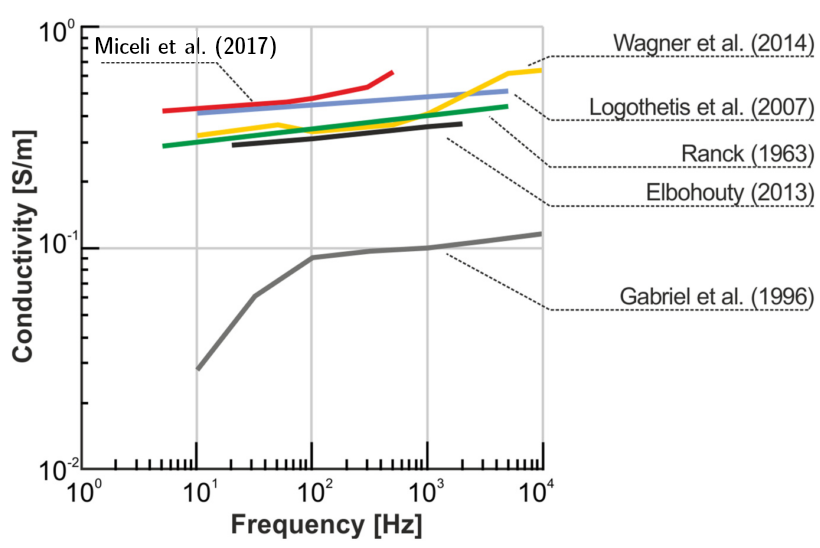
\includegraphics[width=0.6\textwidth]{frequency_dependence}
\end{center}
\caption{\textbf{Literature review of reported conductivities in various species and experimental setups.} 
Most studies seem to indicate a very weak frequency dependence of the extracellular conductivity, which would have a negligible effect on measured extracellular potentials \citep{Miceli2017}. The very low and strongly frequency dependent values measured by \cite{Gabriel1996} represents an outlier, and although it has received substantial attention, it has to the best of our knowledge not been reproduced by any other study.
For details about the data, see \citep{Miceli2017}, and references therein \citep{Ranck1963, Gabriel1996, Logothetis2007, Elbohouty2013, Wagner2014}
}
\label{fig:freq_dep}
\end{figure}



Volume conductor theory is the fundament for forward modeling of extracellular potentials at different spatial scales, from extracellular spikes, LFPs and MUAs, to ECoGs and EEGs. In the following sections we shall review previous modeling works, and insights from simulating electrical potentials at these different scales.
We use the software LFPy \citep{Linden2014, Hagen2018, Hagen2019}, which has volume conductor theory incorporated and can in principle be used to compute extracellular potentials on arbitrarily large spatial scales, surrounding arbitrarily large neuronal populations. 


\section{Single-cell contributions to extracellular potentials}
%\ghnote{Suggest that we start these sections by explaining what $\phi$ tells us at this level. Also, we should refer to the VC-theory and explain which of the assumptions (1-6) that were relaxed in the specific case.}

%\ghnote{Maybe not use current-conservation as a main topic, but rather talk about how extracellular potentials reflect morphology. Say something like: The extracellular potential arising from the activity of a single neuron is a reflection of not only its dynamical activity, but also its  morphology, and neurons with a large spatial extension generally give rise to larger extracellular potentials as there will be larger distances between current.}

%\ghnote{Moved current-conservation figure here. I think that we could call it something else. Perhaps the Hay-neuron-example can be integrated with this figure? And perhaps we should name it single-cell contribution to extracellular potential}.

The transmembrane currents of a neuron during some arbitrary neural activity can be used to calculate extracellular potentials, by applying the formalism described in Sec.~\ref{sec:VC_theory}, and in the simplest case eg.~\ref{eq:VCtheory}.
%The extracellular potentials from a single neuron is a reflection of both cellular dynamics and morphology (the spatial structure of the cell). 
Current conservation requires that the transmembrane currents across the entire cellular membrane at any given time sum to zero \citep{Koch1999, Nunez2006}, and since
an excitatory synaptic input generates a current sink (negative current), this will necessarily lead to current sources elsewhere on the cell. This implies that point neurons, that is, neurons with no spatial structure, will have no net transmembrane currents, and hence cause no extracellular potentials (Fig.~\ref{fig:EP_morph}A). The simplest neuron models that are capable of producing extracellular potentials are therefore two-compartment models, which will have two equal but opposite currents, and cause perfectly dipolar extracellular potentials (Fig.~\ref{fig:EP_morph}B).

Multi-compartment neuron models mimicking the complex spatial structure of real neurons will typically give rise to complicated patterns of current sinks and sources (negative and positive currents respectively), leading to complex, but mostly dipolar-like extracellular potentials (Fig.~\ref{fig:EP_morph}C) \citep{Einevoll2013}.
Note that this framework for calculating extracellular potentials is valid both for subthreshold and suprathreshold neural activity, that is, when a cell receives synaptic input that does not trigger, or does trigger an action potential, respectively (Fig.~\ref{fig:EP_morph}, D versus E).

\begin{figure}[!ht]
\begin{center}
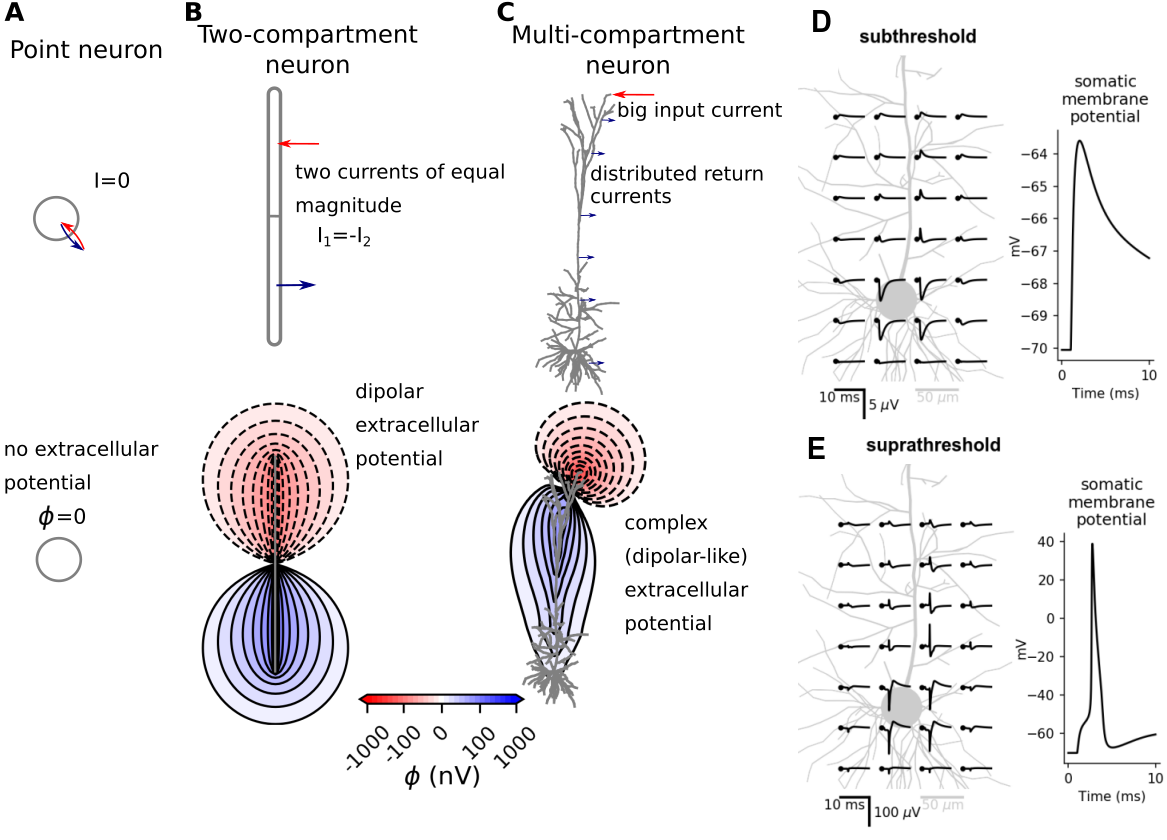
\includegraphics[width=1\textwidth]{single_cell_EP}
\end{center}
\caption{\textbf{Single-cell contributions to the extracellular potential.} 
{\bf A}: Point neurons have no net currents (top), and therefore cause no extracellular potentials (bottom). 
{\bf B}: Two-compartment neuron models have two opposite currents
of identical magnitude (top), and cause perfectly dipolar extracellular potentials (bottom). 
{\bf C}: Multi-compartment neuron models \citep{Hay2011} give rise to complex source-sink patterns (top) and complex (but mostly dipolar-like) extracellular potentials (bottom). 
{\bf D, E}: A single somatic synaptic input to a complex multi-compartment cell model, either subthreshold (D) or suprathreshold (E; double synaptic weight of D), illustrating that the same framework can be used to calculate both the LFP contribution from subthreshold synaptic input, and extracellular action potentials. 
\snnote{Top row, panel B: "two currentS". Top row, panel C: "distributed return currentS".}
}
\label{fig:EP_morph}
\end{figure}

\section{Intra-cortical extracellular potentials from neural populations}
Extracellular potentials measured within neural tissue are often split into two separate frequency domains, which reflect different aspects of the underlying neural activity. 
The low frequency part, that is, the local field potential (LFP), is thought to mostly reflect synaptic input to populations of pyramidal cells, while the high-frequency part, that is, the multi-unit activity (MUA), reflects the population spiking activity (Fig.~\ref{fig:LFP_MUA}).

\begin{figure}[!ht]
\begin{center}
\includegraphics[width=1\textwidth]{population_LFP_MUA.png}
%\includegraphics[width=1\textwidth]{PC_versus_IN}
\end{center}
\caption{\textbf{Extracellular potentials from different waves of synaptic input}. Different brain signals from separate waves of synaptic input to 10 000 layer 5 pyramidal cells from rat \citep{Hay2011}.
{\bf A}: A subset of 100 pyramidal cells, with the LFP electrode locations indicated in the center (colored dots).
{\bf B}: Depth-resolved synaptic inputs arrive in three waves, first targeting the basal dendrites (t=$\sim$60~ms), then the apical dendrites (t=$\sim$130~ms), and lastly uniformly across the entire depth (t=$\sim$200~ms). Note that all synaptic input is pre-defined, that is, there is no network activity.
{\bf C}: The extracellular potential at different depths (colors correspond to dots in panel A), including both spikes and synaptic input.
{\bf D}: The LFP, that is, a low-pass filtered version of the raw signal in C.
{\bf E}: The MUA, that is, a high-pass filtered version of the raw signal in C.
{\bf F}: The MUA, that is, a high-pass filtered, rectivifed and low-pass filtered version of the raw signal in C.
}
\label{fig:LFP_MUA}
\end{figure}


\subsection{Local field potentials}
\tvnnote{Find place to put sentence or two on importance of correlation.}
The LFP is the low-frequency part ($\lesssim$ 500~Hz) of the extracellular potentials, and it is among the oldest and most used brain signals in neuroscience \citep{Einevoll2013}. The LFP is expected to be dominated by large numbers of synaptic inputs to populations of geometrically aligned neurons \citep{Nunez2006, Linden2011, Einevoll2013b}.
In cortex and hippocampus, neurons can broadly speaking be divided into two main classes: the inhibitory interneurons, and the excitatory pyramidal neurons. Pyramidal neurons typically have a clear axis of orientation, that is, the apical dendrites of close-by pyramidal neurons tend to be oriented in the same direction (Fig.~\ref{fig:LFP_MUA}A). This geometrical alignment is important because the LFP contributions from the individual pyramidal cells also align and therefore sum constructively.  For example, basal excitatory synaptic input (Fig.~\ref{fig:LFP_MUA}B, time marked by red line) generates a current sink and corresponding negative LFP deflection in the basal region, and simultaneously a current source and corresponding positive LFP deflection in the apical region (Fig.~\ref{fig:LFP_MUA}D, time marked by red line), while apical excitatory synaptic input leads to the reversed pattern (Fig.~\ref{fig:LFP_MUA}B,D, time marked by blue line). 
Importantly, this means that excitatory input that simultaneously targets both the apical and the basal dendrite will give opposite source/sink patterns which will lead to substantial cancellation and a weak LFP contribution (Fig.~\ref{fig:LFP_MUA}B, D, time marked by orange line).
The same arguments also apply to inhibitory synaptic inputs, with the signs of the currents and LFPs reversed. 

Note that, for example, the LFP signature of apical excitatory synaptic input is inherently similar to that of basal inhibitory input, and indeed, separating between cases like this pose a real challenge in interpreting LFP signals \citep{Linden2010}. 

In contrast to pyramidal neurons, interneurons often lack any clear orientational specificity, meaning that the current dipoles do not align, leading to negligible contribution to LFP signals, except indirectly through giving synaptic input to pyramidal cells \citep{Hagen2016, Telenczuk2016}.

It has been demonstrated that correlations among the synaptic inputs to pyramidal cells can amplify the LFP signal power by orders of magnitude, with the implication that populations receiving correlated synaptic input can dominate the LFP also 1-2~mm outside of the population \citep{Linden2011, Leski2013}.

Although the LFP is believed to predominantly reflect synaptic inputs, active conductances may also contribute to its shaping. Especially slower conductances may play a key role in this, such as long-lasting after-hyperpolarization currents \cite{Reimann2013}, calcium spikes \cite{Suzuki2017}, or the hyperpolarization-activated cation channel I$_{\rm h}$ \cite{Ness2016, Ness2018}. Action potentials are typically expected to contribute little to cortical LFP signals for several reasons \citep{Einevoll2013, Haider2016}, for example, their very short duration with both positive and negative phases (Fig.~\ref{fig:EP_morph}E) would require extreme synchrony to sum constructively in the LFP, and their high frequency content is to a large degree removed from LFPs during low-pass filtering. Note however, that in the hippocampus the highly synchronized spikes found during sharp wave ripples are expected to strongly shape the LFP \citep{Schomburg2012, Luo2018}. 

\subsubsection*{Other approaches}
\tvnnote{Make this section one sentence in LFP}.
Kernels \citep{Hagen2016}

Proxies \cite{Mazzoni2015}

LFP Kernels from experimental spike-triggered averages (Destexhe?)

\subsection{MUA}
While LFPs are thought to mainly reflect the synaptic input to large populations of pyramidal neurons, the multi-unit activity (MUA) can be used to probe the population spiking activity \citep{Pettersen2008}. This can be useful, as some cell-types, like stellate cells and interneurons are expected to have very weak LFP contributions \citep{Linden2011}, but might still be measureable through their spiking activity. Similarly, spatially uniformly distributed synaptic input to pyramidal neurons results in a negligible LFP contribution (Fig.~\ref{fig:LFP_MUA}C, time marked by orange line), while the population might still contribute substantially to the MUA through the extracellular action potentials (Fig.~\ref{fig:LFP_MUA}E-F, time marked by orange line).



%%%%%%%%%%%%%%%%%%%%%%%%%%%%%%%%%%%%%%
%%%%%%%%%%%%%%%%%%%%%%%%%%%%%%%%%%%%%%
%%%%%%%%%%%%%%%%%%%%%%%%%%%%%%%%%%%%%%
\section{ECoG and EEG}
%%%%%%%%%%%%%%%%%%%%%%%%%%%%%%%%%%%%%%
%%%%%%%%%%%%%%%%%%%%%%%%%%%%%%%%%%%%%%
%%%%%%%%%%%%%%%%%%%%%%%%%%%%%%%%%%%%%%
\label{sec:EEG}
\sntxt{
In order to measure \emph{electric potentials in the immediate vicinity of neurons} \slntxt{(OR: LFP and MUA signals)}, we need to insert sharp electrodes into the brain. This highly invasive technique is quite common in animal studies, but can only be applied to humans when there is a clear medical need, for example in patients with intractable epilepsy \citep{Zangiabadi2019}. Fortunately, electric potentials generated by neural activity extend beyond neural tissue and can be picked up by electrodes placed on the brain surface or on top of the scalp. The first technique is known as electrocorticography (ECoG), while the second refers to the non-invasive method of electroencephalography (EEG).

Since EEG electrodes are located relatively far away from the neuronal sources, the current dipole approximation, Eq.~\eqref{eq:CDA}, combined with some head model, can be applied for computing EEG signals \citep{Nunez2006}. By collapsing the transmembrane currents of a neuron simulation into one single current dipole moment, see Eq.~\eqref{dipole}, we can calculate EEG from arbitrary neural activity (Fig.~\ref{fig:multimodal}).

The current dipole approximation is however not an obvious candidate for computing ECoG signals, as the ECOG electrodes are located too close to the signal sources, see \citep{Hagen2018}.




}

%LFP signals are measured inside different brain structures, in the immediate vicinity of the current sources that are causing the LFP signals. A disadvantage with this is that it is invasive, in the sense that electrodes must be inserted into the brain tissue which can only be done in humans when there is a clear medical need, like for patients with intractable epilepsy [cite]. However, the current sources that are causing the LFP signals are also causing measurable electrical signals at the brain surface, called electrocorticography (ECoG), and outside of the head, called electroencephalograpy (EEG) (Fig.~\ref{fig:multimodal}).

%\tvnnote{Should we substantially shorten the above paragraph and remove equations?}
%
%
%\tvnnote{Write breifly about how we can calculate EEGs from arbitrary neural activity} 
%We can calculate EEG from arbitrary neural activity (Fig. \ref{fig:EEG_MEG}).


\begin{figure}[!ht]
\begin{center}
\includegraphics[width=0.5\textwidth]{population_EEG_MEG_cut.png}
%\includegraphics[width=1\textwidth]{PC_versus_IN}
\end{center}
\caption{\textbf{Extracellular potentials from different waves of synaptic input}. Different brain signals from separate waves of synaptic input to 10 000 layer 5 pyramidal cells from rat \citep{Hay2011}.
{\bf A}: The four-sphere head model with two orientations of the neural population, either radial, mimicing a population in a gyrus (top) or tangential, mimicing a population in a sulcus (bottom).
{\bf B}: A snapshot of the EEG signal at the head surface for apical input (time marked with blue dotted line in Fig. \ref{fig:LFP_MUA}), for a radial population (top) or tangential population (bottom).
}
\label{fig:EEG_MEG}
\end{figure}



\subsection{Head models}
\sntxt{
Electric potentials measured on the scalp surface will be affected by the geometries and conductivities of the different constituents of the head \citep{Nunez2006}. This can be incorporated in our EEG calculations by applying simplified or more complex head models.
A well-known simplified head model is the analytical four-sphere model, consisting of four conentric shells representing brain tissue, cerebrospinal fluid (CSF), skull and scalp, where the conductivity can be set individually for each shell \citep{Naess2017, Srinivasan1998, Nunez2006} (Fig.~\ref{fig:head_models}A).
More complex head models make use of high-resolution anatomical MRI-data to map out a geometrically detailed head volume conductor. The link between current dipoles in the brain and resulting EEG signals is determined applying numerical methods such as the finite element method \citep{Larson2013, Logg2012}. Once this link is established we can in principle insert a dipole representing arbitrary neural activity into such a model, and compute the resulting EEG signals quite straightforwardly. The New York Head model is an example of one such pre-solved complex head model, see Fig.~\ref{fig:head_models} \citep{Huang2016}.


The head models introduce no essential frequency filtering of the EEG signal \citep{Pfurtscheller1975, Ranta2017}, however, substantial spatial filtering will occur (Fig.~\ref{fig:foursphere_contour}).
The relatively large size of the EEG electrodes will also contribute to spatial summation of the EEG signals [cite?].
}

%
%Can use analytic four-sphere (Fig. \ref{fig:head_models}A) \citep{Hagen2018, Naess2017}
%Can also used pre-solved complex head models, like the New York head (Fig. \ref{fig:head_models}B) \citep{Huang2016}.
%
%No important frequency  filtering on EEG signal by head \citep{Pfurtscheller1975, Ranta2017}, however, substantial spatial filtering (Fig.~\ref{fig:foursphere_contour}).

\begin{figure}[!ht]
\begin{center}
\includegraphics[width=1.0\textwidth]{4o_contour}
%\includegraphics[width=1\textwidth]{PC_versus_IN}
\end{center}
\caption{\textbf{Effect of head inhomogeneities}.
The same current dipole will give substantially different potentials on the head surface when the different conductivities of the head is included.
}
\label{fig:foursphere_contour}
\end{figure}

\tvnnote{Write something about the spatial filtering from electrode size.}
\snnote{Torbjorn: Was it something in the means of the last sentence above, that you had in mind? Or do  Do you have any suggestions for papers to cite?}


\begin{figure}[!ht]
\begin{center}
\includegraphics[width=1\textwidth]{head_models.png}
\end{center}
\caption{\textbf{[placeholder] Head models} A: Four-sphere. B: New York head model.
\snnote{I'm going to fix this fig!}
}
\label{fig:head_models}
\end{figure}





\section{Inverse modelling}
\tvnnote{Gaute will write}
CSD

EEG dipoles

Spke sorting

Since MUAs and LFPs reflect different aspects of neural activity, they can be used in combination to gain additional insights, as is for example done in Laminar Population Analysis \citep{Einevoll2007, Blomquist2009}.

\section{Software tools}
LFPy etc.
\tvnnote{Recycle text from LFPy 2.0 paper about other softwares (sec 4.7.}
\tvnnote{Maybe we don't need this section? Just say that 'here we've used LFPy'}

Typically split into two separate tasks: Simulate neural activity, mostly relying on the NEURON simulator \citep{Hines1997}, through the Python interface \citep{Hines2009}. Extracellular potentials are then calculated from these currents, through volume conductor theory. 


\section{Summary and Discussion}
\label{sec:summary}
In this chapter, we reviewed the theory for modelling extracellular potentials. Starting at the level of extracellular ionic movements, we showed how neuronal activity gives rise to electrical fluctuations that can be picked up at various spatial scales ranging from the local of MUA and LFP scale to the more global scale of ECoG and EEG. We further reviewed how recorded signals at these various spatial scales can be interpreted in terms of how various features in the recorded signals reflect various aspects of neuronal activity. In brief, the MUA reflects the spiking activity of nearby neurons, the LFP reflect the distribution of synaptic inputs to nearby neuronal populations, while ECoG and EEG reflect the same as the LFP, but on a larger spatial scale. 

We note that there are several related measurement modalities that were not considered here, including magnetoencephalograpy (MEG), voltage-sensitive dye imaging (VSDI), calcium imaging, functional magnetic resonance imaging (fMRI) and positron emission tomography (PET). Of these, the MEG is expected to originate from the same process at LFP, ECoG and EEG signals (Fig.~\ref{fig:multimodal}), i.e., from synaptic input to geometically aligned populations of pyramidal neurons \citep{Hamalainen1993}, and can be modeled with similar approaches as those reviewed above. However, because of the nature of magnetic fields, MEG is most sensitive to populations that are tangential to the head surface, instead of radial (see Fig. \ref{fig:EEG_MEG}). VSDI and calcium imaging reflect the reflecting area-weighted neuronal membrane potentials and intracellular calcium dynamics, which and are in principle easily accessed variables in neuronal simulations, while fMRI and PET reflect blood supply and metabolic cost, which are typically not explicitly included in models. 
 

\begin{enumerate}
 \item Summary of chapter
 \item Ongoing large-scale projects (HBP, Allen)
 \subitem Using LFP in constraining models?
 \item Brain-Machine interfaces?
 \item Where to go?
 \subitem fMRI, VSD, Ca img.
\end{enumerate}

\section{Other brain signals}
\tvnnote{Massive shortening}

\subsection*{Magnetoencephalograpy (MEG)}




%%%%%%%%%%%%%%%%%%%%%%%%%%%%%%%%%%%%%%%%%%%%%%%%%%
%%%%%%%%%%%%%%%%%%%%%%%%%%%%%%%%%%%%%%%%%%%%%%%%%%

\section*{Acknowledgements}
\label{sec:acknowledgements}
This research has received funding from the European Union Horizon 2020 Framework Programme for Research
and Innovation under Specific Grant Agreement No. 785907 (Human Brain Project SGA2), the Research Council of Norway (Notur, nn4661k), and \tvnnote{INCF?}



%%%%%%%%%%%%%%%%%%%%%%%%%%%%%%%%%%%%%%%%%%%%%%%%%%
%%%%%%%%%%%%%%%%%%%%%%%%%%%%%%%%%%%%%%%%%%%%%%%%%%

\section*{References}
\label{sec:bibliography}
\bibliography{ECS_bookchapter.bib}

%%%%%%%%%%%%%%%%%%%%%%%%%%%%%%%%%%%%%%%%%%%%%%%%%%
%%%%%%%%%%%%%%%%%%%%%%%%%%%%%%%%%%%%%%%%%%%%%%%%%%


\end{document}  
